\chapter{An Empirical Study}

Excluding Dixon's factorization method, all attacks analyzed so far exploit
some peculiarities of a candidate RSA public key $\angular{N, e}$ in order to
recover the private exponent.
Summarizingly:
\begin{itemize}
  \item Pollard's $p-1$ attack works only if the predecessor of any of
    the two primes factorizing the public modulus is composed of very small
    primes;
  \item  Williams' $p+1$ attack works under similar conditions - the predecessor
    or the successor of any of the two primes can be easily factorized;
  \item Fermat's factorization is valuable whenever the two primes $p$ and $q$
    are really close to each other;
  \item Pollard's $\rho$ method is best whenever one of the two primes is
    strictly lower than the other.
\end{itemize}
Dixon's factorization method instead, being a general-purpose factorization
algorithm, can be employed to \emph{measure} the strength of a RSA
keypair: the more relations (satisfying \ref{eq:dixon:fermat_revisited}) are
found, the less it is assumed resistant.

Given these hypotesis, it has been fairly easy to produce valid RSA candidates
that are exploitable using the above attacks, and use them to assert the
correctness of the implementation.

On the top of that, there has been a chance to test the software under real
conditions: we choose download the SSL keys (if any) of the top one million visited
websites, and survey them with the just developed software. This not only gave
us the opportunity to survey the degree of security on which the internet is
grounded today, but also led to a deeper understanding of the capacities and limits of
the most widespread libraries offering crypto nowadays.

\vfill
\section{To skim off the dataset}

What has been most scandalous above all was to discover was that more than
\strong{half} of the most visited websites do \strong{not} provide SSL
connection over port 443 - reserved for HTTPS according to IANA
\cite{iana:ports}.
To put it in numbers, we are talking about $533$ thousands websites either
unresolved or unreachable in $10$ seconds.
As a side note for this, many websites (like \texttt{baidu.com} or
\texttt{qq.com}) keep a tcp connection open without writing anything to the
channel, requiring us to adopt a combination of non-blocking socket with the
\texttt{select()} system call in order to drop any empty communication.
It would be intesting to investigate more on these facts, asking ourselves how
many of those unsuccessful connetion are actually wanted from the server, and
how many dropped for cernsorship reasons; there's enough room for another
project.

Of the remaining $450,000$ keys, $21$ were using different ciphers than RSA. All
others represent the dataset upon which we worked on.

\section{To count}

Once all valuable certificate informations have been stored inside a database,
almost any query can be performed to get a statistically valuable dregree of
magnitude to which some conditions are satisfied. What follows now is a list of
commented examples that we believe are relevant parameters for understanding of
how badly internet is configured today.

\begin{figure}[H]
  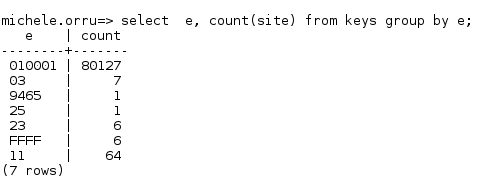
\includegraphics[width=0.7\textwidth]{e_count.png}
\end{figure}

The most prolific number we see here, $65537$ in hexadecimal, is the fouth
Fermat number and no other than the largest known prime of the form $2^{2^n} +
1$. Due to its composition, it has been advised by NIST as default public
exponent, and successfully implemented in most softwares, such as \openssl\!.

Sadly, a negleglible number of websites is using low public exponents,
which makes the RSA key vulnerable to Coppersmith's attack. Unfortunately, this
topic goes beyond the scope of this research and hence has not been analyzed
further.

\begin{figure}[H]
  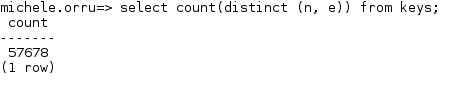
\includegraphics[width=0.7\textwidth]{n_count.png}
\end{figure}

What is interesting to see here is that an enormous portion of our dataset
shared the same public key, pushing down our of one order of magnitude the
number of expected keys. Reasons for this are mostly practical: it is extremely
frequent to have blogs hosted on third-party sercives such as ``Blogspot'' or
``Wordpress'' which always provide the same X.509 certificate, as they belong to
an unique organization.
Though improbable, it is even possible that exists a millesimal portion of
different websites sharing the same public key due to a
bad CSRNG, and therefore also the same private key. Such a case has been
already investigated in \cite{ron:whit}.

\begin{figure}[H]
  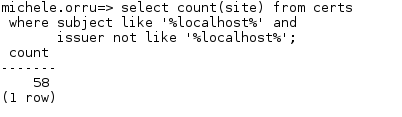
\includegraphics[width=0.6\textwidth]{localhost_certs.png}
\end{figure}

Here we go. A suprisingly consistent nuber of websites provides certificates
with dummy, wrong, or even testing informations. Some even inject non-printable
bytes in the \emph{common name} field.
Some are certified from authorities, some chinese governmental entities.



\chapter{Conclusions \label{conclusions}}
\noindent
Everytime we see a certificate, we get this idea the somebody is telling us the
connection is safe. There is some authority out there telling what to do.
We should be thinking more about what these authorities are and what they are
doing.

%%% Local Variables:
%%% mode: latex
%%% TeX-master: "question_authority"
%%% End:
